% !TEX program = pdflatex
% ------------------------------------------------------------
% ITKA2004 Databases & Data Management
% Lecture 6 (90 min): Relational Algebra
% Theme: metropolis (matches earlier lectures)
% ------------------------------------------------------------
\documentclass[10pt,aspectratio=169]{beamer}

\usetheme[
  progressbar=frametitle,
  numbering=fraction
]{metropolis}

% --- Packages
\usepackage[utf8]{inputenc}
\usepackage{booktabs}
\usepackage{amsmath}
\usepackage{amssymb}
\usepackage{tikz}
\usetikzlibrary{positioning,arrows.meta,shapes.geometric}
\usepackage{qtree}
\usepackage{graphicx}

\usetikzlibrary{positioning,arrows.meta,shapes.geometric,shapes.callouts}
\setkeys{Gin}{width=\linewidth,height=0.70\textheight,keepaspectratio}

% ------------------------------------------------------------
% Footer (Metropolis)
% ------------------------------------------------------------
\setbeamertemplate{frame footer}{%
  \tiny Michael Emmerich (Professor, PS Fellow)\hfill Databases Spring 2026\hfill Faculty of Information Technology, University of Jyväskylä%
}

% --- Metadata
\title{Databases and Data Management}
\subtitle{Lecture 6: Relational Algebra}
\author{Michael Emmerich (Professor, PS Fellow)}
\institute{Faculty of Information Technology\\University of Jyväskylä}
\date{Spring 2026}

% --- Small title graphic
\titlegraphic{%
  \begin{tikzpicture}[remember picture,overlay]
    \node[anchor=south east,opacity=0.10] at ([xshift=-2mm,yshift=2mm]current page.south east) {%
      \begin{tikzpicture}[scale=0.75]
        \draw[rounded corners=6pt,line width=2pt] (0,0) rectangle (5,3);
        \draw[line width=2pt] (0.6,2.4) -- (4.4,2.4);
        \node at (2.5,1.6) {\Large RA};
      \end{tikzpicture}
    };
  \end{tikzpicture}%
}

% --- Convenience macros
\newcommand{\select}{\sigma}
\newcommand{\proj}{\pi}
\newcommand{\rename}{\rho}

\begin{document}

\maketitle

% ------------------------------------------------------------
\begin{frame}{Why Relational Algebra (RA)? (motivation)}
\begin{itemize}
  \item RA is \textbf{operational}: it describes \emph{how} a query can be computed.
  \item SQL queries can be translated to RA and then \textbf{optimized} for speed (equivalences + indexes).
  \item RA operator names (JOIN, DIVISION, \dots) are standard in DBMS literature and query optimizers.
  \item \textbf{Join operations} will be used later to motivate \textbf{normal forms} and anomalies.
  \item You already know SQL is \textbf{relationally complete}; RA clarifies \textbf{what queries can/cannot be computed}.
  \item Querying in RA-like form exists in practice in some systems / tools (historically e.g. MS Access alternatives).
\end{itemize}
\end{frame}

\begin{frame}{Learning goals}
By the end of this lecture you should be able to:
\begin{enumerate}
  \item distinguish declarative vs operational query languages
  \item define the core RA operators and read their notation
  \item formulate and understand RA queries (incl.\ joins and division)
  \item apply equivalence transformations (push \(\sigma,\pi\), join associativity)
  \item explain how SQL engines use RA trees for execution plans
\end{enumerate}
\end{frame}

\begin{frame}{Outline}
\tableofcontents
\end{frame}

% ------------------------------------------------------------
\section{Introduction}

\begin{frame}{Relational Algebra in one slide}
\begin{itemize}
  \item Query languages allow \textbf{retrieval and manipulation} of database data.
  \item Query languages \(\neq\) programming languages:
  \begin{itemize}
    \item not intended to be Turing-complete
    \item focus on \textbf{easy, efficient access} to large datasets
  \end{itemize}
\end{itemize}
\end{frame}

\begin{frame}{Relational query languages: algebra vs calculus}
Two mathematical query languages are foundational:
\begin{itemize}
  \item \textcolor{blue}{Relational Algebra (RA)}: operational, step-by-step computation
  \item \textcolor{brown}{Relational Calculus / SQL}: declarative, specify \emph{what} result you want
\end{itemize}
\end{frame}

\begin{frame}{Basic constraints and syntax in RA}
\begin{itemize}
  \item RA operators operate on \textbf{relation instances} (schema + set of tuples).
  \item A RA query takes relations as input and returns a relation.
  \item Output \textbf{schema depends only} on input schemas and operator parameters.
  \item Notation:
  \begin{itemize}
    \item \textbf{positional} (field numbers): useful for formal definitions (e.g., renaming)
    \item \textbf{named-field}: more readable; use whenever possible
  \end{itemize}
\end{itemize}
\end{frame}

\begin{frame}{Core operators (overview)}
\begin{itemize}
  \item Basic operators:
  \begin{itemize}
    \item Selection \(\select_c(R)\) \hfill \texttt{SIGMA\_(c)(R)}
    \item Projection \(\proj_{a_1,\dots,a_k}(R)\) \hfill \texttt{PI\_(a1,...,ak)(R)}
    \item Cross product \(R \times S\) \hfill \texttt{R X S}
    \item Renaming \(\rename(R)\) \hfill \texttt{r\_(x -> y)(R)}
    \item Set difference \(R \setminus S\) \hfill \texttt{R - S}
    \item Union \(R \cup S\) \hfill \texttt{R U S}
  \end{itemize}
  \item Derived but very useful:
  \(\cap\), joins (\(\Join\), \(\Join_c\), \(\Join_{a_1,\dots,a_k}\)), division \((/)\)\\
  \hspace*{1.2em}\texttt{R INTERSECT S, R JOIN S, R JOIN\_(c) S, R JOIN\_(a1,...,ak) S, P / R}
  \item Closure: each operator returns a relation \(\Rightarrow\) expressions compose.
\end{itemize}
\end{frame}

% ------------------------------------------------------------
\section{Operators}

% ------------------------------------------------------------
\begin{frame}{Example instance (s, r, b) used in this lecture}
\small
\begin{columns}[T,onlytextwidth]
\column{0.73\textwidth}
\textbf{Consider a boat reservation database.}

\[
s=\begin{array}{|c|c|c|c|}\hline
sid&sname&age&rating\\\hline
22&dustin&35&7\\
31&lubber&55&8\\
44&guppy&35&5\\\hline
\end{array}
\qquad
r=\begin{array}{|c|c|c|}\hline
sid&bid&day\\\hline
22&101&2026-02-01\\
22&102&2026-02-03\\
31&102&2026-02-02\\\hline
\end{array}
\qquad
b=\begin{array}{|c|c|}\hline
bid&color\\\hline
101&red\\
102&green\\
103&red\\\hline
\end{array}
\]

\vspace{0.4em}
\footnotesize
\textbf{Schemas:}\\[-0.2em]
\texttt{Sailors S(sid,sname,age,rating)}\\
\texttt{Reservations R(sid,bid,day)}\\
\texttt{Boats B(bid,color)}

\column{0.27\textwidth}
\centering
\vspace{3cm}
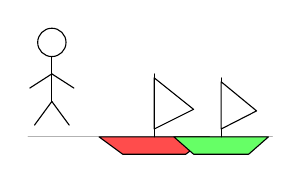
\begin{tikzpicture}[x=1cm,y=1cm, line cap=round, line join=round]
% Stickman
\begin{scope}[shift={(0.0,1.0)}]
  \draw (0,0) circle (0.18);
  \draw (0,-0.18) -- (0,-0.75);
  \draw (0,-0.40) -- (-0.28,-0.58);
  \draw (0,-0.40) -- (0.28,-0.58);
  \draw (0,-0.75) -- (-0.22,-1.05);
  \draw (0,-0.75) -- (0.22,-1.05);
\end{scope}

% Water line
\draw[gray!60] (-0.3,-0.2) -- (2.8,-0.2);

% Red boat (bid 101,103)
\begin{scope}[shift={(0.6,-0.2)}]
  \fill[red!70] (0,0) -- (1.4,0) -- (1.1,-0.22) -- (0.3,-0.22) -- cycle;
  \draw (0,0) -- (1.4,0) -- (1.1,-0.22) -- (0.3,-0.22) -- cycle;
  \draw (0.70,0) -- (0.70,0.80);
  \fill[white] (0.70,0.75) -- (0.70,0.10) -- (1.20,0.35) -- cycle;
  \draw (0.70,0.75) -- (0.70,0.10) -- (1.20,0.35) -- cycle;
\end{scope}

% Green boat (bid 102)
\begin{scope}[shift={(1.55,-0.2)}]
  \fill[green!60] (0,0) -- (1.2,0) -- (0.95,-0.22) -- (0.25,-0.22) -- cycle;
  \draw (0,0) -- (1.2,0) -- (0.95,-0.22) -- (0.25,-0.22) -- cycle;
  \draw (0.60,0) -- (0.60,0.75);
  \fill[white] (0.60,0.70) -- (0.60,0.10) -- (1.05,0.33) -- cycle;
  \draw (0.60,0.70) -- (0.60,0.10) -- (1.05,0.33) -- cycle;
\end{scope}
\end{tikzpicture}
\end{columns}
\end{frame}


% ------------------------------------------------------------
\begin{frame}{Selection \(\select_{c(a_1,\dots,a_n)}(R)\)}
\begin{itemize}
  \item \textcolor{blue}{Semantics:} keep only tuples that satisfy condition \(c\).
  \item \textcolor{blue}{Syntax:} \(S=\select_{c(a_1,\dots,a_n)}(R)\).
  \item \textcolor{blue}{ASCII (quiz):} \texttt{SIGMA\_(c)(R)}    (Why? S in SIGMA stands for selection)
\end{itemize}

\vspace{0.4em}
\small
\[
s=\begin{array}{|c|c|c|c|}\hline
sid&sname&age&rating\\\hline
22&dustin&35&7\\
31&lubber&55&8\\
44&guppy&35&5\\\hline
\end{array}
\qquad
\select_{age<50}(s)=
\begin{array}{|c|c|c|c|}\hline
sid&sname&age&rating\\\hline
22&dustin&35&7\\
44&guppy&35&5\\\hline
\end{array}
\]
\end{frame}

% ------------------------------------------------------------
\begin{frame}{Projection \(\proj_{a_1,\dots,a_k}(R)\)}
\begin{itemize}
  \item \textcolor{blue}{Semantics:} keep only listed columns, then remove duplicates.
  \item \textcolor{blue}{Syntax:} \(S = \proj_{a_1,\dots,a_k}(R)\).
  \item \textcolor{blue}{ASCII (quiz):} \texttt{PI\_(a1,...,ak)(R)}    (Why: P in PI stands for \textit{Projection})
\end{itemize}

\vspace{0.4em}
\small
\[
s=\begin{array}{|c|c|c|c|}\hline
sid&sname&age&rating\\\hline
22&dustin&35&7\\
31&lubber&55&8\\
44&guppy&35&5\\\hline
\end{array}
\qquad
\proj_{age}(s)=
\begin{array}{|c|}\hline
age\\\hline
35\\
55\\\hline
\end{array}
\]
\small Duplicate ages are removed (set semantics).
\end{frame}

% ------------------------------------------------------------
\begin{frame}{Union, intersection, set difference}
\begin{itemize}
  \item \textcolor{blue}{Syntax:} \(R \ \textbf{op}\ S\), union-compatible schemas,
        \(\textbf{op}\in\{\cup,\cap,\setminus\}\).
  \item \textcolor{blue}{Semantics:} set operations over tuples.
  \item \textcolor{blue}{ASCII (quiz):}
        \texttt{R U S}, \texttt{R INTERSECT S}, \texttt{R - S}
\end{itemize}

\vspace{0.4em}
\small
Let
\[
r_1=\select_{bid=101}(r),\quad r_2=\select_{bid=102}(r)
\]
\[
r_1=\begin{array}{|c|c|c|}\hline
sid&bid&day\\\hline
22&101&2026-02-01\\\hline
\end{array}
\quad
r_2=\begin{array}{|c|c|c|}\hline
sid&bid&day\\\hline
22&102&2026-02-03\\
31&102&2026-02-02\\\hline
\end{array}
\]
\[
r_1\cup r_2=
\begin{array}{|c|c|c|}\hline
sid&bid&day\\\hline
22&101&2026-02-01\\
22&102&2026-02-03\\
31&102&2026-02-02\\\hline
\end{array}
\]
\end{frame}

\begin{frame}{Intersection \(\cap\): example}
\small
Sailors who reserved boat 101 \emph{and} boat 102:
\[
\proj_{sid}(\select_{bid=101}(r))\ \cap\ \proj_{sid}(\select_{bid=102}(r))
\]
\[
\proj_{sid}(\select_{bid=101}(r))=\begin{array}{|c|}\hline sid\\\hline 22\\\hline\end{array}
\quad
\proj_{sid}(\select_{bid=102}(r))=\begin{array}{|c|}\hline sid\\\hline 22\\31\\\hline\end{array}
\]
\[
=\begin{array}{|c|}\hline sid\\\hline 22\\\hline\end{array}
\]
\end{frame}

\begin{frame}{Set difference \(\setminus\): example}
\small
Sailors with no reservations:
\[
\proj_{sid}(s)\setminus \proj_{sid}(r)
\]
\[
\proj_{sid}(s)=\begin{array}{|c|}\hline sid\\\hline 22\\31\\44\\\hline\end{array}
\qquad
\proj_{sid}(r)=\begin{array}{|c|}\hline sid\\\hline 22\\31\\\hline\end{array}
\qquad
=\begin{array}{|c|}\hline sid\\\hline 44\\\hline\end{array}
\]
\end{frame}

% ------------------------------------------------------------
\begin{frame}{Cross product \(R \times S\)}
\begin{columns}[T,onlytextwidth]
\column{0.46\textwidth}
\begin{itemize}
  \item \textcolor{blue}{Syntax:} \(T = R \times S\)
  \item \textcolor{blue}{Semantics:} all combinations of tuples; concatenate attributes
  \item Size: \(|R \times S| = |R|\cdot|S|\) (can explode quickly)
  \item In Example:  \(3\times 3=9\) rows; in real DBs this can be huge.
  \item \textcolor{blue}{ASCII (quiz):} \texttt{R X S}
\end{itemize}

\column{0.54\textwidth}
\small
\[
\proj_{sid,sname}(s)=
\begin{array}{|c|c|}\hline
sid&sname\\\hline
22&dustin\\
31&lubber\\
44&guppy\\\hline
\end{array}
\qquad
\proj_{bid}(b)=
\begin{array}{|c|}\hline
bid\\\hline
101\\102\\103\\\hline
\end{array}
\]
\[
\proj_{sid,sname}(s)\times \proj_{bid}(b)=
\begin{array}{|c|c|c|}\hline
sid&sname&bid\\\hline
22&dustin&101\\22&dustin&102\\22&dustin&103\\
31&lubber&101\\31&lubber&102\\31&lubber&103\\
44&guppy&101\\44&guppy&102\\44&guppy&103\\\hline
\end{array}
\]
\end{columns}
\end{frame}

% ------------------------------------------------------------
\begin{frame}{Renaming \(\rename\)}
\begin{itemize}
  \item Avoid attribute-name clashes (self-joins, products/joins with overlapping names).
  \item \textcolor{blue}{Syntax (named-field):} \(\rename_{a\rightarrow a'}(R)\) (conceptually).
  \item \textcolor{blue}{Syntax (positional):}
        \(S=\rename_{i_1\rightarrow a'_{i_1},\dots,i_k\rightarrow a'_{i_k}}(R)\).
  \item \textcolor{blue}{ASCII (quiz):} \texttt{RHO\_(x -> y)(R)} (R in RHO stands for \textit{\textbf{R}enaming})
\end{itemize}

\vspace{0.4em}
\small
We want to compare sailors with each other, so we create two copies and rename:
\[
s_1=\rename_{sid\rightarrow sid1,\;age\rightarrow age1}(s),
\quad
s_2=\rename_{sid\rightarrow sid2,\;age\rightarrow age2}(s)
\]
\[
s_1=\begin{array}{|c|c|c|c|}\hline
sid1&sname&age1&rating\\\hline
22&dustin&35&7\\
31&lubber&55&8\\
44&guppy&35&5\\\hline
\end{array}
\quad
s_2=\begin{array}{|c|c|c|c|}\hline
sid2&sname&age2&rating\\\hline
22&dustin&35&7\\
31&lubber&55&8\\
44&guppy&35&5\\\hline
\end{array}
\]
\end{frame}
% ------------------------------------------------------------
\begin{frame}{Theta join \(\Join_{c}\)}
\begin{itemize}
  \item \textcolor{blue}{Syntax:} \(R \Join_{c(a_1,\dots,a_n)} S\)
  \item \textcolor{blue}{Semantics:} select from the product:
  \[
  R \Join_c S \;=\; \select_c(R\times S)
  \]
  \item Practical convention: use relation aliases in self-joins.
  \item \textcolor{blue}{ASCII (quiz):} \texttt{R JOIN\_(c) S}
\end{itemize}

\vspace{0.4em}
\small
Older-than relation (who is older than whom):
\[
t=s_1\Join_{age1>age2}s_2
\]
\[
\proj_{sid1,age1,sid2,age2}(t)=
\begin{array}{|c|c|c|c|}\hline
sid1&age1&sid2&age2\\\hline
31&55&22&35\\
31&55&44&35\\\hline
\end{array}
\]
\small Only sailor 31 (age 55) is older than 22 and 44 (age 35).
\end{frame}

% ------------------------------------------------------------
\begin{frame}{Self-join example: one-stop train connection}
\small
Schema:
\[
Train(origin,destination,start\_time,arrival\_time)
\]

\begin{itemize}
  \item Goal: find connections from \texttt{Jyvaskyla} to \texttt{Oulu}
        with exactly one intermediate stop \texttt{X}.
  \item Constraint: the second train must depart after the first arrives:
        \(s2 > a1\).
\end{itemize}

\vspace{0.4em}
Rename two copies (self-join preparation):
\[
t_1=\rename_{origin\rightarrow o1,\ destination\rightarrow d1,\ start\_time\rightarrow s1,\ arrival\_time\rightarrow a1}(Train)
\]
\[
t_2=\rename_{origin\rightarrow o2,\ destination\rightarrow d2,\ start\_time\rightarrow s2,\ arrival\_time\rightarrow a2}(Train)
\]

Self-join query (intermediate stop is where \(d1=o2\)):
\[
\proj_{d1,s1,a1,s2,a2}\Big(
\select_{o1='Jyvaskyla'\ \wedge\ d2='Oulu'}\big(
t_1\Join_{d1=o2\ \wedge\ s2>a1} t_2
\big)\Big)
\]
\end{frame}


% ------------------------------------------------------------
\begin{frame}{Self-join execution on an instance}
\scriptsize
\begin{columns}[T,onlytextwidth]
\column{0.55\textwidth}
Example instance:
\[
Train=
\begin{array}{|c|c|c|c|}\hline
origin&destination&start\_time&arrival\_time\\\hline
Jyvaskyla&Tampere&08{:}00&10{:}30\\
Tampere&Oulu&11{:}10&14{:}40\\
Jyvaskyla&Seinajoki&09{:}00&10{:}20\\
Seinajoki&Oulu&10{:}10&13{:}00\\
Seinajoki&Oulu&10{:}40&13{:}30\\\hline
\end{array}
\]

\vspace{0.4em}
\centering
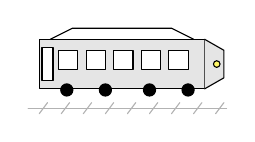
\begin{tikzpicture}[x=1cm,y=1cm, line cap=round, line join=round]
% Simple train icon (text-free)
\begin{scope}[scale=0.7]
  % tracks
  \draw[gray!60] (-0.2,-0.35) -- (3.4,-0.35);
  \foreach \x in {0.0,0.4,0.8,1.2,1.6,2.0,2.4,2.8,3.2} {
    \draw[gray!60] (\x,-0.45) -- (\x+0.15,-0.25);
  }

  % body
  \fill[gray!20] (0,0) rectangle (3.0,0.9);
  \draw (0,0) rectangle (3.0,0.9);

  % nose
  \fill[gray!20] (3.0,0) -- (3.35,0.2) -- (3.35,0.7) -- (3.0,0.9) -- cycle;
  \draw (3.0,0) -- (3.35,0.2) -- (3.35,0.7) -- (3.0,0.9);

  % roof
  \draw (0.2,0.9) -- (0.6,1.1) -- (2.4,1.1) -- (2.8,0.9);

  % windows
  \foreach \x in {0.35,0.85,1.35,1.85,2.35} {
    \fill[white] (\x,0.35) rectangle (\x+0.35,0.70);
    \draw (\x,0.35) rectangle (\x+0.35,0.70);
  }

  % door
  \fill[white] (0.05,0.15) rectangle (0.25,0.75);
  \draw (0.05,0.15) rectangle (0.25,0.75);

  % wheels
  \foreach \x in {0.5,1.2,2.0,2.7} {
    \fill[black] (\x,-0.02) circle (0.11);
    \draw (\x,-0.02) circle (0.11);
  }

  % headlight
  \fill[yellow!60] (3.22,0.45) circle (0.06);
  \draw (3.22,0.45) circle (0.06);
\end{scope}
\end{tikzpicture}

\column{0.45\textwidth}
Execution idea:
\begin{enumerate}
  \item Pair rows where \(d1=o2\) (same stop).
  \item Keep pairs with feasible transfer \(s2>a1\).
  \item Filter endpoints: \(o1='Jyvaskyla'\), \(d2='Oulu'\).
  \item Output stop and times.
\end{enumerate}

\vspace{0.3em}
Result:
\[
\begin{array}{|c|c|c|c|c|}\hline
X&s1&a1&s2&a2\\\hline
Tampere&08{:}00&10{:}30&11{:}10&14{:}40\\
Seinajoki&09{:}00&10{:}20&10{:}40&13{:}30\\\hline
\end{array}
\]

Rejected pair:
\texttt{Jyvaskyla->Seinajoki (arr 10:20)} with
\texttt{Seinajoki->Oulu (dep 10:10)} fails \(s2>a1\).
\end{columns}
\end{frame}


% ------------------------------------------------------------
\begin{frame}{Equi-join and natural join \texorpdfstring{($\bowtie$)}{(bowtie)}}
\begin{columns}[T,onlytextwidth]
% ---------------- left column: equi-join
\column{0.50\textwidth}
\small
\textbf{Equi-join}

\begin{itemize}
  \item \textbf{Definition:} \(R \bowtie_{a_1,\dots,a_k} S\) joins on equality of
        the listed attributes; duplicate join columns removed.
  \item \textbf{ASCII:}\\[-0.2em]
        \texttt{R JOIN\_(a1,...,ak) S}
\end{itemize}

\vspace{0.2em}
\scriptsize
\[
\begin{aligned}
s \bowtie_{sid} r &=\\[-0.6em]
&\begin{array}{|c|c|c|c|c|c|}\hline
sid&sname&age&rating&bid&day\\\hline
22&dustin&35&7&101&2026-02-01\\
22&dustin&35&7&102&2026-02-03\\
31&lubber&55&8&102&2026-02-02\\\hline
\end{array}
\end{aligned}
\]
\scriptsize Join on equality of \texttt{sid}; one \texttt{sid} column remains.

% ---------------- right column: natural join
\column{0.50\textwidth}
\small
\textbf{Natural join}

\begin{itemize}
  \item \textbf{Definition:} \(R \bowtie S\) is an equi-join on \emph{all}
        common attribute names; duplicates removed.
  \item \textbf{ASCII:}\\[-0.2em]
        \texttt{R JOIN S}
\end{itemize}

\vspace{0.2em}
\scriptsize
\[
\begin{aligned}
r \bowtie b &=\\[-0.6em]
&\begin{array}{|c|c|c|c|}\hline
sid&bid&day&color\\\hline
22&101&2026-02-01&red\\
22&102&2026-02-03&green\\
31&102&2026-02-02&green\\\hline
\end{array}
\end{aligned}
\]
\scriptsize \quad \qquad Common name is \texttt{bid} here \\
\quad \qquad (watch unintended common names).
\end{columns}
\end{frame}


% ------------------------------------------------------------
% Join examples (more variety) -- UPDATED with explicit renaming
\begin{frame}{Join examples: theta join (non-equality)}
\small
Schema reminders:
\[
s(sid,sname,age,rating),\quad r(sid,bid,day)
\]

\begin{itemize}
  \item Pair each sailor with each reservation made by a \textbf{different} sailor:
  \[
  s \Join_{s.sid \neq r.sid} r
  \]

  \item Self-join: pairs where one sailor is \textbf{older} than another.

  \smallskip
  First create two renamed copies:
  \[
  s_1=\rename_{sid\rightarrow sid1,\;age\rightarrow age1}(s),\qquad
  s_2=\rename_{sid\rightarrow sid2,\;age\rightarrow age2}(s)
  \]

  Then join them and project the ids:
  \[
  \proj_{sid1,sid2}\big(s_1 \Join_{age1>age2} s_2\big)
  \]
\end{itemize}
\end{frame}


\begin{frame}{Join examples: equi-join (explicit keys)}
\small
Assume:
\[
s(sid,sname,age),\quad r(sid,bid,day),\quad b(bid,color)
\]
\begin{itemize}
  \item Sailor names with reserved boat colors:
  \[
  \proj_{sname,color}\big((s \Join_{sid} r)\Join_{bid} b\big)
  \]
  \item Same idea including reservation day:
  \[
  \proj_{sname,color,day}\big((s \Join_{sid} r)\Join_{bid} b\big)
  \]
\end{itemize}
\end{frame}

\begin{frame}{Join examples: self-join for “exists” / “comparison” queries}
\small
Schema:
\[
s(sid,sname,age,rating)
\]
\begin{itemize}
  \item Sailors who are \textbf{not the youngest} (someone is younger):
  \[
  \proj_{sid1,sname}\big(s_1 \Join_{age1>age2} s_2\big)
  \]
  \item Sailors who share the \textbf{same age} with someone else:
  \[
  \proj_{sid1,sname}\big(s_1 \Join_{age1=age2 \wedge sid1\neq sid2} s_2\big)
  \]
\end{itemize}
\small (Here \(s_1=\rename_{sid\rightarrow sid1,age\rightarrow age1}(s)\), similarly for \(s_2\).)
\end{frame}

% ------------------------------------------------------------
\section{Division}

% ------------------------------------------------------------
\begin{frame}{Division \(P / R\)}
\begin{itemize}
  \item Intuition: \textbf{find the \(x\)-tuples that are related to all \(y\)-tuples}.
  \item Let \(P(x_1,\dots,x_m,y_1,\dots,y_k)\) and \(R(y_1,\dots,y_k)\).
  \item Result \(S = P/R\) has schema \((x_1,\dots,x_m)\).
  \item Here \(\mathbf{x}\circ \mathbf{y}\) means \textbf{concatenation of tuples}
        (append the \(y\)-components to the \(x\)-components).
\end{itemize}

\small
\[
P/R=\{\,\mathbf{x}\in \proj_{x_1,\dots,x_m}(P)\mid
\mbox{for all }\mathbf{y}\in R,\ \mbox{exists }\mathbf{p}\in P:
\mathbf{p}=\mathbf{x}\circ \mathbf{y}\,\}
\]

\small
\textbf{Sanity check (why it feels like division):}\\[-0.2em]
If \(A(x)\) and \(B(y)\), then \((A \times B)/B = A\), because every \(x\in A\)
pairs with every \(y\in B\) in \(A \times B\).
\end{frame}


\begin{frame}{Division: the “FOR ALL” operator (pattern)}
Division answers queries of the form:
\[
\text{Find } x \text{ such that for \emph{all} } y \in Y,\ (x,y)\in P.
\]
\begin{itemize}
  \item Template:
  \[
  \text{Answer} = P \; / \; Y
  \]
  \item If you see “\textbf{for every} required thing”, think division.
  \item Example: Find students in S who have completed all courses in C
  \item Example: Find sailors with age higher than all other sailors
\end{itemize}
\end{frame}

% ------------------------------------------------------------
% Division example (richer): sailors who reserved boats of ALL colors present
\begin{frame}{Division \(/ \): richer instance (reserved all colors present)}
\small
\textbf{Goal:} sailors who have reserved boats of \emph{all colors} that appear in the boat instance.

\smallskip
We first build a relation of \emph{(sid,color)} pairs that the sailor has actually reserved:
\[
p=\proj_{sid,color}(r \Join_{bid} b)
\]
and the set of \emph{required colors}:
$
y=\proj_{color}(b)
$
\[
p=\begin{array}{|c|c|}\hline
sid&color\\\hline
22&red\\
22&green\\
31&green\\\hline
\end{array}
\qquad
y=\begin{array}{|c|}\hline
color\\\hline
red\\
green\\\hline
\end{array}
\]
Now division returns those sids that are paired with \emph{every} color in \(y\):
\[
p/y=
\begin{array}{|c|}\hline
sid\\\hline
22\\\hline
\end{array}
\]

\smallskip
\small Interpretation: only sailor 22 has at least one reservation of a red boat and at least one reservation of a green boat.
\end{frame}


\begin{frame}{Youngest sailor(s) using division (idea)}
\begin{itemize}
  \item Reformulate: “find sailors whose age is \(\le\) the age of \emph{all} sailors”.
  \item Build \(p(sid1,sid2)\) meaning: sailor \(sid1\) is \textbf{younger or equal} than sailor \(sid2\).
  \item Then keep those \(sid1\) that relate to \emph{all} \(sid2\) via division.
\end{itemize}

\small
\[
s_1=s,\quad s_2=s,\quad
p=\proj_{sid1,sid2}\Big(\rename_{sid\rightarrow sid1,\,age\rightarrow age1}(s_1)\Join_{age1\le age2}\rename_{sid\rightarrow sid2,\,age\rightarrow age2}(s_2)\Big)
\]
\[
youngest \;=\; p\; /\; \proj_{sid2}\big(\rename_{sid\rightarrow sid2}(s)\big)
\]
\end{frame}

\begin{frame}{Youngest sailor(s) using division (with our instance)}
\small
From the instance \(s\) (ages: 35, 55, 35) obtain \textit{(Exercise: Write in RA using $\sigma$, $\rho$ and $\times$):)}
\[
p(sid1,sid2)=\{(sid1,sid2)\mid age(sid1)\le age(sid2)\}
\] 
\[
p=\begin{array}{|c|c|}\hline
sid1&sid2\\\hline
22&22\\
22&31\\
22&44\\
31&31\\
44&22\\
44&31\\
44&44\\\hline
\end{array}
\quad
\proj_{sid2}(s_2)=\begin{array}{|c|}\hline sid2\\\hline 22\\31\\44\\\hline\end{array}
\]
\[
p/\proj_{sid2}(s_2)=
\begin{array}{|c|}\hline sid1\\\hline 22\\44\\\hline\end{array}
\]
\small So the youngest sailors are \(sid=22\) and \(sid=44\) (both age 35).
\end{frame}

\begin{frame}{Division using only basic operators (optional)}
Let \(P(X,Y)\) and \(R(Y)\). Then:
\[
P / R \;=\; \proj_X(P)\; \setminus\; \proj_X\big( (\proj_X(P)\times R)\; \setminus\; P \big)
\]
\begin{itemize}
  \item Start with all candidate \(X\) values
  \item Remove those for which \emph{some required \(Y\)} is missing
  \item This implements “for all” using set difference
\end{itemize}
\end{frame}

% ------------------------------------------------------------
\section{More examples (for self-study)}

\begin{frame}{Examples of RA queries}
Assume:
\[
s(sid,sname,rating,age),\quad r(sid,bid,day),\quad b(bid,color)
\]
\begin{itemize}
  \item Names and ages of sailors with rating \(>4\):
  \[
  \proj_{sname,age}(\select_{rating>4}(s))
  \]
  \item sids of sailors who have at least one reservation:
  \[
  \proj_{sid}(s \Join_{sid} r)
  \]
  \item sids of sailors with no reservation:
  \[
  \proj_{sid}(s)\setminus \proj_{sid}(r)
  \]
\end{itemize}
\end{frame}

\begin{frame}{Union vs intersection (boats example)}
\small
\begin{itemize}
  \item sids of sailors who reserved \textbf{green OR red} boats:
  \[
  \proj_{sid}(\select_{color=green}(r\Join b))\ \cup\ \proj_{sid}(\select_{color=red}(r\Join b))
  \]
  \item sids of sailors who reserved \textbf{green AND red} boats:
  \[
  \proj_{sid}(\select_{color=green}(r\Join b))\ \cap\ \proj_{sid}(\select_{color=red}(r\Join b))
  \]
\end{itemize}
\end{frame}

\begin{frame}{Early selection/projection usually wins}
\small
\begin{example}
Find \((sid,sname)\) of sailors who reserved a green boat:
\[
\proj_{sid,sname}\big(\select_{color='green'}(s \Join (r \Join b))\big)
\]
Alternative (push projection and selection):
\[
\proj_{sid,sname}\Big(s \Join \big(\proj_{sid,bid}(r)\Join \select_{color='green'}(b)\big)\Big)
\]
\end{example}
Rule of thumb: \textbf{select and project as early as possible.}
\end{frame}

\begin{frame}{Practice prompts (quick in-class mini-examples)}
Try to write RA for:
\begin{enumerate}
  \item Names of sailors who reserved a \textbf{green} boat \emph{and} a \textbf{red} boat.
  \item sids of sailors who reserved \textbf{at least one} boat \emph{but not} boat 101.
  \item sids of sailors who reserved \textbf{all} red boats (division).
\end{enumerate}
\end{frame}

% ------------------------------------------------------------
\section{Composition, equivalences, and RA trees}

\begin{frame}{Equivalence of RA expressions}
\begin{definition}
Two RA expressions \(E\) and \(F\) are equivalent (written \(E\equiv F\)) iff for all valid inputs: \(E = F\).
\end{definition}
\begin{example}
\[
A\cap B \equiv A\setminus (A\setminus B)
\qquad
\select_{a=10\wedge b=a}(A)\equiv \select_{a=b}(\select_{b=10}(A))
\]
\end{example}
\end{frame}

\begin{frame}{Important equivalences (optimizer staples)}
\begin{itemize}
  \item Associativity of join:
  \[
  A\Join(B\Join C)\equiv (A\Join B)\Join C
  \]
  \item Push selection:
  \[
  \select_{C(B)}(A\Join B)\equiv A\Join \select_{C(B)}(B)
  \]
  \item Push projection (keep join attributes):
  \[
  \proj_{S(A)}(A\Join B)\equiv \proj_{S(A)}\big(A\Join \proj_{S(B)}(B)\big)
  \]
  \item Heuristic: push \(\sigma\) and \(\pi\) to reduce intermediate results.
\end{itemize}
\end{frame}

\begin{frame}{RA trees}
RA expressions can be represented as \textbf{RA trees} (evaluate bottom-up).
\begin{example}
\[
b \Join (r \Join \select_{age\le 40}(s))
\quad\leadsto\quad
\Tree[.$\Join$ b [.$\Join$ r [.$\sigma_{age\le 40}$ s ] ] ]
\]
\end{example}
Leaves are relations; inner nodes are operators.
\end{frame}

\begin{frame}{Join trees explode: many equivalent plans}
For \(A\Join B\Join C\Join D\), different join trees are equivalent but may have very different costs:
\[
\Tree[.$\Join$ [.$\Join$ [.$\Join$ A B ] C ] D ]
\equiv
\Tree[.$\Join$ [.$\Join$ A [.$\Join$ B C ] ] D ]
\equiv
\Tree[.$\Join$ [.$\Join$ A B ] [.$\Join$ C D ] ]
\]
\end{frame}

\begin{frame}{Catalan numbers (how many join trees?)}
The number of full binary join trees for \(m\) relations is the Catalan number \(C_{m-1}\):
\[
C_0=1,\qquad C_n=\sum_{i=0}^{n-1} C_i C_{n-i-1}
\]
Growth is rapid \(\Rightarrow\) optimizers use heuristics + cost estimation.
\end{frame}

\begin{frame}{SQL to RA (core SELECT-FROM-WHERE)}
\begin{itemize}
  \item SQL pattern:
  \[
  \texttt{SELECT }a_1,\dots,a_k\ \texttt{ FROM }R_1,\dots,R_m\ \texttt{ WHERE }C
  \]
  \item RA translation:
  \[
  \proj_{a_1,\dots,a_k}\Big(\select_C(R_1\times \cdots \times R_m)\Big)
  \]
  \item One possible RA tree (right-deep):
  \vspace{-0.6cm}
  \[
  \Tree[.$\pi_{a_1,\dots,a_k}$ [.$\sigma_C$ [.$\times$ $R_1$ [.$\vdots$ [.$\times$ $R_{m-1}$ $R_m$ ] ] ] ] ]
  \]
\end{itemize}
\end{frame}

\begin{frame}{Query optimization (big picture)}
\begin{itemize}
  \item DBMS translates SQL \(\rightarrow\) an initial RA tree.
  \item Optimizer explores equivalent RA trees (algebraic rules).
  \item It estimates cost using statistics + available \textbf{indexes}.
  \item Chosen plan becomes the \textbf{query execution plan}.
\end{itemize}
\end{frame}

\begin{frame}{Relational vs Turing completeness}
\begin{itemize}
  \item A language is \textbf{relationally complete} if it can compute everything RA can compute.
  \item A language is \textbf{Turing complete} if it can compute any computable function (like C).
  \item Turing complete \(\Rightarrow\) relationally complete, but not vice versa.
  \item RA is \textbf{not} Turing complete.
  \item Example beyond plain RA: \textbf{transitive closure} (reachability in graphs).
  \item SQL is relationally complete and adds more (aggregation, grouping, etc.).
\end{itemize}
\end{frame}

\begin{frame}{Extended relational algebra (beyond classical RA)}
Classical RA includes \(\sigma,\pi,\Join,\cup,\setminus,\times,\rho,/\) (set-based).

\vspace{0.4em}
DBMS often use \textbf{extended RA} to model SQL features:
\begin{itemize}
  \item \textbf{Outer joins} (LEFT/RIGHT/FULL OUTER JOIN): keep non-matching tuples with NULLs
  \item \textbf{Aggregation and grouping}: \(\gamma\) (group-by), e.g., COUNT, SUM, AVG, MIN, MAX
  \item Often also: sorting and LIMIT as physical/plan operators
\end{itemize}

\vspace{0.4em}
\small We focus on classical RA for clarity; later we connect it to SQL features used in practice.
\end{frame}

% ------------------------------------------------------------
\section{Wrap-up}

\begin{frame}{Summary and outlook}
\begin{itemize}
  \item RA: core operators \(\setminus,\cup,\proj,\select,\times,\rename\); derived \(\cap,\Join,/\).
  \item Many equivalent formulations exist; optimizers rely on equivalences.
  \item Heuristics: push \(\sigma,\pi\); join ordering is hard (large search space).
  \item Next: connect joins and decomposition ideas to \textbf{normal forms}.
\end{itemize}
\end{frame}



% \begin{frame}{Joke slide: Hash join vs hash joint}
% \textbf{Student:} “I optimized my query with a \emph{hash joint}.”\\[0.5em]
% \textbf{DBMS:} “A hash \textbf{join}.”\\[0.5em]
% \textbf{Student:} “Right… a hash join.”\\[0.5em]
% \textbf{DBMS:} “Good. Because a hash \emph{joint} is what you need after proving \(\sigma\) pushdown for the 12th time.”\\[0.7em]
% \small (Summary: push \(\sigma\) and \(\pi\) early, choose good joins, and don’t do \(\times\) unless you mean it.)
% \end{frame}


\begin{frame}{Joke slide: division and join}

% --- Text-free TikZ picture (stick figures + smashed tables)
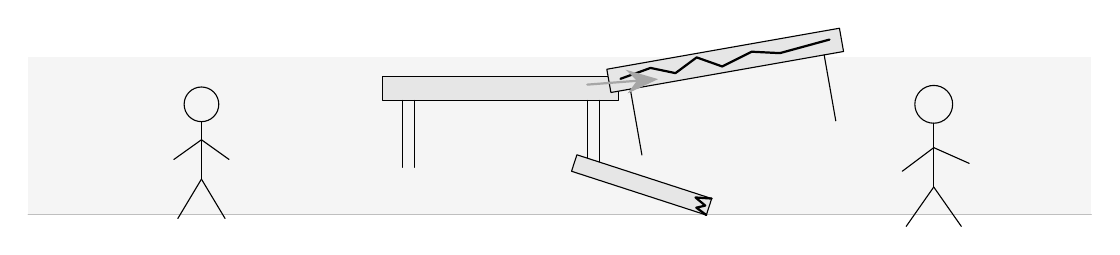
\begin{tikzpicture}[x=1cm,y=1cm, line cap=round, line join=round]
\definecolor{tbl}{RGB}{230,230,230}
\definecolor{floor}{RGB}{245,245,245}

% Floor
\fill[floor] (-0.3,-2.2) rectangle (13.2,-0.2);
\draw[gray!50] (-0.3,-2.2) -- (13.2,-2.2);

% Intact table (left)
\fill[tbl] (4.2,-0.75) rectangle (7.2,-0.45);
\draw (4.2,-0.75) rectangle (7.2,-0.45);
\draw (4.45,-0.75) -- (4.45,-1.60);
\draw (6.95,-0.75) -- (6.95,-1.60);
\draw (4.60,-0.75) -- (4.60,-1.60);
\draw (6.80,-0.75) -- (6.80,-1.60);

% Smashed-into table (right, slightly rotated)
\begin{scope}[shift={(7.1,-0.65)}, rotate=10]
  \fill[tbl] (0,0) rectangle (3.0,0.30);
  \draw (0,0) rectangle (3.0,0.30);
  \draw (0.25,0) -- (0.25,-0.85);
  \draw (2.75,0) -- (2.75,-0.85);
  % Crack/jagged line
  \draw[thick] (0.15,0.15) -- (0.55,0.22) -- (0.85,0.10) -- (1.15,0.25)
               -- (1.45,0.08) -- (1.85,0.20) -- (2.20,0.12) -- (2.85,0.18);
\end{scope}

% Broken half-table piece (foreground)
\begin{scope}[shift={(6.6,-1.65)}, rotate=-18]
  \fill[tbl] (0,0) rectangle (1.8,0.22);
  \draw (0,0) rectangle (1.8,0.22);
  % Rough broken edge
  \draw[thick] (1.8,0) -- (1.65,0.05) -- (1.75,0.11) -- (1.60,0.17) -- (1.8,0.22);
\end{scope}

% Impact arrow
\draw[-{Stealth[length=4mm]}, thick, gray!70] (6.8,-0.55) -- (7.7,-0.48);

% Child (left stick figure)
\begin{scope}[shift={(1.9,-0.8)}]
  \draw (0,0) circle (0.22);
  \draw (0,-0.22) -- (0,-0.95);
  \draw (0,-0.45) -- (-0.35,-0.70);
  \draw (0,-0.45) -- (0.35,-0.70);
  \draw (0,-0.95) -- (-0.30,-1.45);
  \draw (0,-0.95) -- (0.30,-1.45);
\end{scope}

% Mother (right stick figure)
\begin{scope}[shift={(11.2,-0.8)}]
  \draw (0,0) circle (0.24);
  \draw (0,-0.24) -- (0,-1.05);
  \draw (0,-0.55) -- (-0.40,-0.85);
  \draw (0,-0.55) -- (0.45,-0.75);
  \draw (0,-1.05) -- (-0.35,-1.55);
  \draw (0,-1.05) -- (0.35,-1.55);
\end{scope}
\end{tikzpicture}

\vspace{0.6em}
\small
\small
\textbf{A mess} has appeared in the kitchen. One kitchen table is smashed
into another, and a table is broken in half.\\[0.6em]

\textbf{Child:} "The teacher was telling us how to \textbf{\textit{divide}} tables by using other tables."\\[0.4em]
\textbf{Mother:} "Oh no..."\\[0.4em]
\textbf{Child:} "But don't worry, mother. Our teacher also told us also how to \textbf{\textit{join}} the tables again."\\
\end{frame}

\end{document}
